\documentclass{standalone}
\usepackage{tikz}
\begin{document}
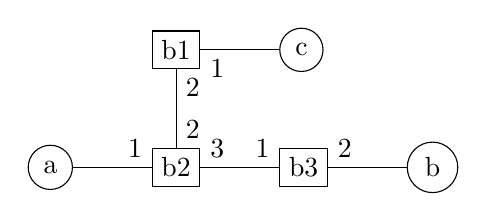
\begin{tikzpicture}
    \draw

    (0,0) node [draw, circle, anchor=east]{a}
    --++(1,0)node[above left]{1} node [draw, rectangle, anchor=west](b2){b2}
    (b2.east)node[above right]{3}--++(1,0)node[above left]{1} node [draw, rectangle, anchor=west](b3){b3}
    (b3.east)node[above right]{2}--++(1,0) node [draw, circle, anchor=west]{b}
    (b2.north)node[above right]{2}--++(0,1)node[below right]{2} node [draw, rectangle, anchor=south](b1){b1}
    (b1.east)node[below right]{1}--++(1,0)node [draw, circle, anchor=west]{c}
    ;
\end{tikzpicture}
\end{document}